\chapter{\label{chap:implementierung}WIP Implementierung der Prototypen}
In diesem Kaptitel wird nach dem in Kapitel \ref{chap:konzeption} präsentiertem Lösungsweg die detaillierte Beschreibung der technischen Realisierung der Prototypen vorgestellt.\\
\todo{Nach der Beschreibung der Hauptkomponente wird auf die Umsetzung der Offlinefunktionalität und des Konfliktmanagements eingegangen. Im Zuge dessen wird ... vorgestellt...}
%
%
%
\section{WIP Die Kernkomponente Contacts}

Kontakte lesen, anlegen, bearbeiten, löschen
Couch ermittelt Delta über die Revisionsnummer und sendet nur die neuen Daten.
CRUD, toggleEdit, getConflictRevisions, chooseRev()\\
Redux: Contacts= ContactsView, ContactsContainer, reducer/actions
%
%
%
\section{WIP Offlinefunktionalität}
Die Prototypen \it{amilia-qouch} und \it{amilia-rdx} sind vollständig offline verwendbar.
Alle in \autoref{chap:offlinefirst} beschriebenen Grundvoraussetzungen werden von beiden Prototypen erfüllt und sämtliche umgesetzten Funktionen sind sowohl mit als auch ohne Internetverbindung durchführbar.
%
%
% LOCAL DB
%
\sub{Datenspeicherung}
Redux Offline speichert, wie in \autoref{sub:reduxpersist} bereits beschrieben, alle im Redux Store verwalteten Daten im LocalStorage. \autoref{fig:local-rdx} zeigt alle gespeicherten, nutzerInnengenerierten Daten im LocalStorage.
%
\begin{figure}[H]
  \centering
  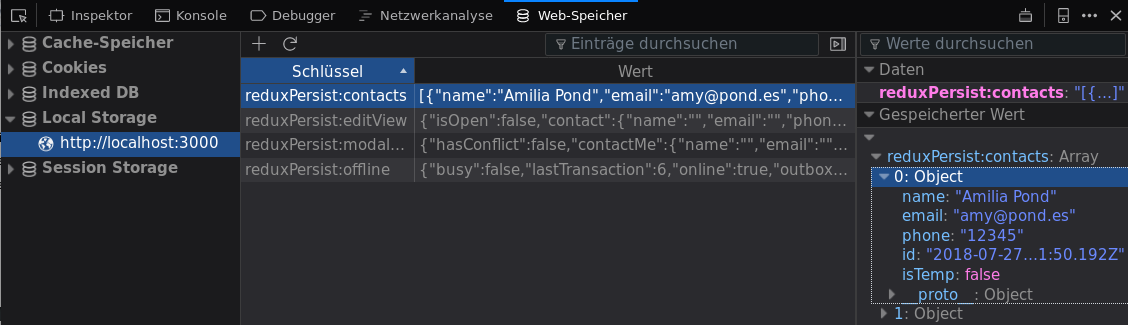
\includegraphics[width=\textwidth]{impl/localRdx}
  \grayRule
  \caption[Gespeicherte Daten im LocalStorage]{Gespeicherte Daten des Prototypen \it{amilia-rdx} im LocalStorage,\\Screenhot: Developer Tools im Firefox Browser}
  \label{fig:local-rdx}
\end{figure}
% 
Der Prototyp \it{amilia-qouch} nutzt zur lokalen Datenspeicherung PouchDB. PouchDB speichert die von NutzerInnen generierten Daten in IndexedDB, vgl. \autoref{chap:pouch}. In \autoref{fig:local-qouch} sind die gespeicherten Daten in der IndexedDB zu sehen.
%
\begin{figure}[H]
  \centering
  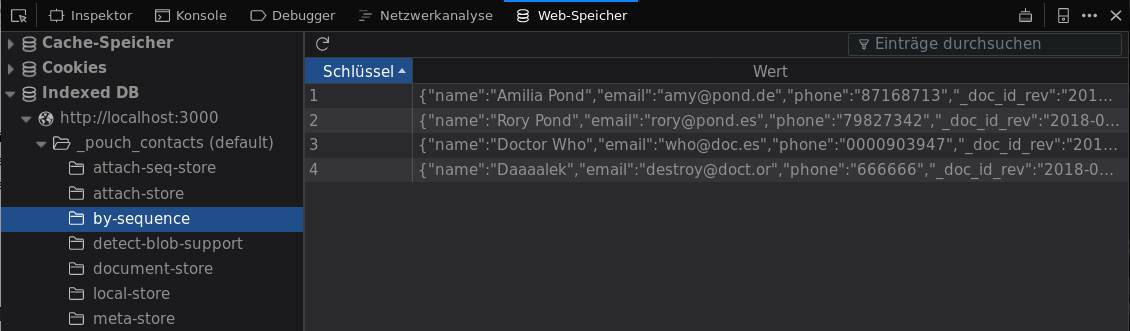
\includegraphics[width=\textwidth]{impl/localQouch}
  \grayRule
  \caption[Gespeicherte Daten in IndexedDB]{Gespeicherte Daten des Prototypen aus \it{amilia-qouch} in IndexedDB,\\Screenhot: Developer Tools im Firefox Browser}
  \label{fig:local-qouch}
\end{figure}
%
% SYNC
%
\sub{Datenbanksynchronisation}
Zwischen PouchDB und CouchDB können Daten in Echtzeit synchronisiert werden. Um die Live--Replikation zu aktivieren, muss im Synchronisationsaufruf der Parameter \tt{live: true} gesetzt sein.
Bricht die Internetverbindung ab, stoppt auch die Synchronisation.
Dank der angegebenen Parameter \tt{retry: true} versucht PouchDB die Synchronisation solange neuzustarten bis die Anwendung wieder mit dem Internet verbunden ist. \autoref{code:sync} zeigt die Implementation der Datenbankensynchronisation im Prototypen \it{amilia-qouch}.
%
\begin{center}
  \lstinputlisting[language=REACT,
  numbers=left,xleftmargin=20pt,
  firstline=1,lastline=5,
  framexleftmargin=15pt,
  caption={Synchronisation zwischen PouchDB und CouchDB im Prototyp \it{amilia-qouch}},
  label=code:sync]{code/sync.js}
\end{center}
Redux Offline nimmt einem auch Arbeit bei der Datensynchronisation ab. Alle Daten die sich im Queue befinden werden automatisch an den Server gesendet, sobald eine Internetverbindung besteht. Das funktioniert jedoch nicht so einfach wenn der Server nicht an ist. In der Dokumentation von Redux Offline steht, dass die Aktion solange versucht wird auszuführen, bis die Anwendung wieder mit dem Internet verbunden ist ~\cite{giving-up}. Allerdings wird die \sc{rollback} Aktion gefeuert wenn der Server nicht verfügbar ist und die Aktion wird abgebrochen.
\begin{center}
  \lstinputlisting[language=REACT,
  numbers=left,xleftmargin=20pt,
  firstline=6,
  framexleftmargin=15pt,
  caption={Discard Konfiguration für amilia-rdx},
  label=code:discard]{code/sync.js}
\end{center}
Die Discard Konfiguration bestimmt wann eine Aktion abgebrochen, und wann sie immer wieder neugestartet wird. Im \autoref{code:discard} ist in den Zeilen 1 bis 4 abzulesen wie diese Konfiguration überschrieben wird. Nun wird die Aktion nur abgebrochen wenn der Server verfügbar ist und einen \gls{HTTP} Status zwischen 400 und 500 zurückgibt.
In den darauffolgenden Zeilen wird die eigens implementierte Konfiguration mit der Standardkonfiguration von Redux Offline zusammengeführt wird.
Alle Daten werden nun auch nach einem Ausfall an den Server gesendet.\\
Im Gegensatz zum \it{amilia-qouch} Prototypen werden die Daten nur in eine Richtung automatisch gesendet. Es gibt keine Implementierung einer automatischen Replikation von den Daten auf dem Server zum lokalen Speicher.
%
%
%
\section{WIP Konfliktmanagement}
Wie kann ein Konflikt erzeugt werden?\\
(manuell -- siehe \ref{sub:detect})
\begin{center}
  \lstinputlisting[language=REACT,
    firstline=1,lastline=12,
    numbers=left,xleftmargin=20pt,framexleftmargin=15pt,
    caption={Laden von konfliktbehafteten Kontakten},
    label=code:conflicts]{code/conflicts.js}
\end{center}

\begin{center}
  \lstinputlisting[language=REACT,
    firstline=14,lastline=38,
    numbers=left,xleftmargin=20pt,framexleftmargin=15pt,
    caption={Laden von konfliktbehafteten Kontakten},
    label=code:conflicts2]{code/conflicts.js}
\end{center}

\begin{center}
  \lstinputlisting[language=REACT,
    firstline=40,lastline=43,
    numbers=left,xleftmargin=20pt,framexleftmargin=15pt,
    caption={Laden von konfliktbehafteten Kontakten},
    label=code:conflicts3]{code/conflicts.js}
\end{center}

Modal:
\begin{figure}[H]
  \centering
  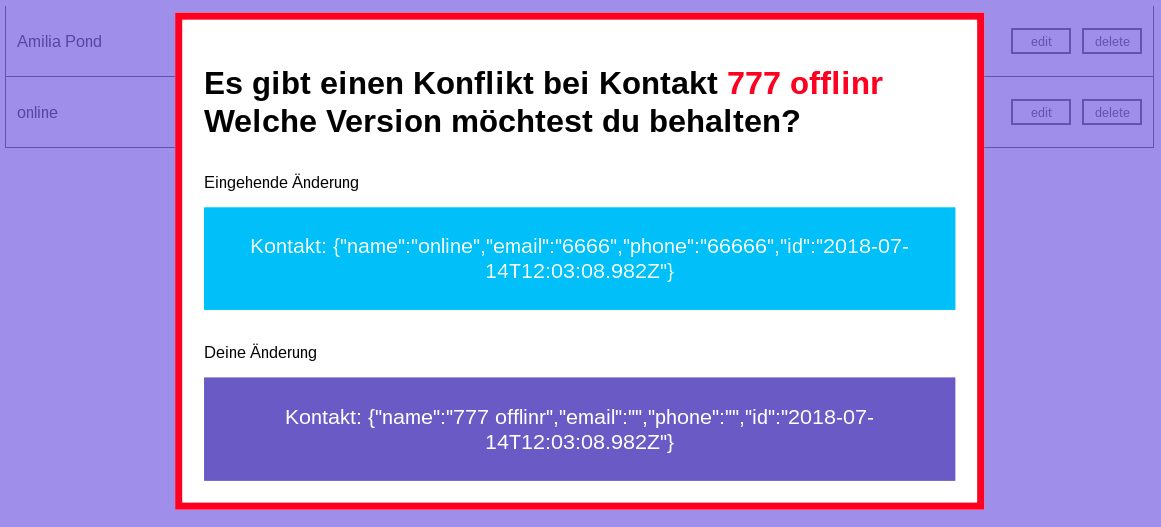
\includegraphics[width=\textwidth]{impl/Modal}
  \grayRule
  \caption{Konfliktdialog in Aktion}
  \label{fig:modal}
\end{figure}
Modal ist nicht bei Redux offline enthalten, das es nicht die Möglichkeit bietet Konflikte zu erkennen, gescheige denn zu speichern.
%
%
%
%
% Installationsanleitung
%
\section{WIP Installationsanleitung}
\todo{build und so}
Beide entwickelten Prototypen sind als öffentliche Repositories auf GitHub\footnote{Software--Entwicklungs--Plattform \url{https://github.com/}} zu finden. 
Um sie zu installieren müssen folgende Schritte ausgeführt werden.
\sub{amilia-qouch}
1. Zuerst muss das Repository kopiert werden:
\lstset{language=sh, caption={},belowcaptionskip=0.3\baselineskip}
\begin{lstlisting}
git clone git@github.com:hulkoba/amilia-qouch.git
# oder
git clone https://github.com/hulkoba/amilia-qouch.git
\end{lstlisting}
2. Dann muss man in das Verzeichnis navigieren und alle Abhängigkeiten installieren.
\begin{lstlisting}
cd amilia-qouch
npm install
\end{lstlisting}
3. Mittels
\begin{lstlisting}
npm start
\end{lstlisting}
wird die Anwendung gestartet.
%
\sub{amilia-rdx}
1. Auch hier muss das Repository zuerst kopiert werden:
\lstset{language=sh, caption={},belowcaptionskip=0.3\baselineskip}
\begin{lstlisting}
git clone git@github.com:hulkoba/amilia-rdx.git
# oder
git clone https://github.com/hulkoba/amilia-rdx.git
\end{lstlisting}
2. Schritt zwei ist identisch mit dem in der \tt{amilia-qouch} Anleitung\\
3. Mittels
\begin{lstlisting}
npm run server
npm start
\end{lstlisting}
wird zuerst der Server, dann die Anwendung gestartet.

%
% Testfälle
%
\section{\label{chap:impl:test}Testfälle}
\section{\label{sec:impl:test}Testfälle}
Folgende Testfälle zur Offlinefunktionalität werden während der Entwicklung stetig durchgeführt. Das erfolgreiche Bestehen dieser Tests ist eine notwendige Qualitätseigenschaft der zu entwickelnden Prototypen.
\begin{description}[leftmargin=0.7cm,style=nextline]
\item[Netzwerkstatus:] 
Die Anwendung muss zu jeder Zeit den korrekten Netzwerkstatus anzeigen.\\
\item[Kontakte lesen:] 
Die Anwendung bei jedem Start die Kontakte aus dem lokalen Speicher oder aus der \it{Datenbank} laden.\\
\item[Kontakt anlegen:] 
Die Anwendung muss zu jedem Zeitpunkt in der Lage sein einen Kontakt mit jedem seiner Attribute anzulegen. Dazu muss er immer lokal gespeichert werden und sobald eine Internetverbindung besteht, persistiert werden.
Das Anlegen eines Kontakts im Offlinestatus ist für die Konfliktforcierung erforderlich.\\
\item[Kontakt bearbeiten:] 
Die Anwendung muss zu jedem Zeitpunkt in der Lage sein einen Kontakt mit jedem seiner Attribute zu bearbeiten. Ist keine Internetverbindung vorhanden, müssen die Änderungen lokal übernommen und später, sobald sich der Netzwerkstatus ändert, synchronisiert werden.
Das Bearbeiten eines Kontakts im Offlinestatus ist für die Konfliktforcierung erforderlich.\\
\item[Kontakt löschen:] 
Die Anwendung muss zu jedem Zeitpunkt in der Lage sein einen Kontakt zu löschen.
Das Löschen eines Kontakts im Offlinestatus ist für die Konfliktforcierung erforderlich.
\end{description}